% This is samplepaper.tex, a sample chapter demonstrating the
% LLNCS macro package for Springer Computer Science proceedings;
% Version 2.21 of 2022/01/12
%
\documentclass[runningheads]{llncs}
%
\usepackage[T1]{fontenc}
% T1 fonts will be used to generate the final print and online PDFs,
% so please use T1 fonts in your manuscript whenever possible.
% Other font encondings may result in incorrect characters.
%
\usepackage{graphicx}
\usepackage{amsmath}
\usepackage{cite}
\usepackage{hyperref}

\usepackage[misc,geometry]{ifsym}

% Used for displaying a sample figure. If possible, figure files should
% be included in EPS format.
%
% If you use the hyperref package, please uncomment the following two lines
% to display URLs in blue roman font according to Springer's eBook style:
%\usepackage{color}
%\renewcommand\UrlFont{\color{blue}\rmfamily}
%\urlstyle{rm}
%
\begin{document}
%
\title{Comparison of approaches to using machine learning models to increase the efficiency of the global search algorithm for solving multicriteria problems\thanks{This work was supported by the Ministry of Science and Higher Education of the Russian Federation, project no. FSWR-2023-0034, and by by the Research and Education Mathematics Centre ``Mathematics for Future Technologies'', project no. 075-02-2024-1439.} }
%
\titlerunning{Algorithms for solving multicriteria problems}
% If the paper title is too long for the running head, you can set
% an abbreviated paper title here
%
\author{Sergey Konnov\orcidID{0009-0003-4590-0870} \and
Evgeny Kozinov \Letter\orcidID{0000-0001-6776-0096} \and
Konstantin Barkalov \Letter\orcidID{0000-0001-5273-2471} \and
Vladimir Grishagin\orcidID{0000-0002-2884-3670}}
%
\authorrunning{S. Konnov, E. Kozinov, K. Barkalov and V. Grishagin}
% First names are abbreviated in the running head.
% If there are more than two authors, 'et al.' is used.

\institute{Lobachevsky State University of Nizhni Novgorod, Nizhni Novgorod, Russia 
\email{a230172@unn.ru}, \email{\{konstantin.barkalov,evgeny.kozinov\}@itmm.unn.ru}, \email{vagris@unn.ru}}
%
\maketitle

%
\begin{abstract}
To solve a multicriteria optimization problem, it is necessary to find a whole set of independent variables corresponding to non-dominated criteria values (Pareto set). The complexity of these problems increases significantly in the case when the criteria are multiextremal. The paper presents several variations of the global optimization algorithm intended for solving black-box multiobjective problems with multiextremal criteria. The developed methods are based on a combination of the information-statistical approach and machine learning procedures aimed at increasing the efficiency of constructing the Pareto set. As a novelty, the paper describes a new approach to using machine learning models within the algorithm of multicriteria optimization. The effectiveness of different versions of the developed algorithm is estimated on the base of  a representative computational experiment.

\keywords{Multicriteria Problems \and Global Optimization \and Machine Learning.}
\end{abstract}
%
%
%
\section{Introduction}
\label{sec:1}

\cite{Miettinen1999,Ehrgott2005,Pardalos2017,ML_MCO_2023,Evtushenko2014,Deb2002,Durillo2010,Mostaghim2007,NDG09,RC05,ZLT01,Gergel2019_2,Gergel2018,GergelKozinov2020,Marler2004,Strongin2000,Sergeyev2013,SVM_2000,PROB_2004,iOpt_url,Grishagin2015_2}

Problems of optimal choice are widespread in many areas of activity. As a rule, in complicated decision making models there are several functions to be optimized which reflect the decision making objectives and those are, in general case, contradictory. In these circumstances, the notion of optimal solution is more complicated than in single criterion (scalar) statement formulated as mathematical programming problem because there exist incomparable decisions. In this situation under introduced definition of domination, the set of non-dominated variants (Pareto set) is taken as the solution of the multiobjective problem.

In our study we deal with methods for solving the most complex class of multicriteria problems where criteria are considered as ``black-box'' functions and are multiextremal \cite{Miettinen1999,Ehrgott2005,Pardalos2017,Strongin2000,Sergeyev2013}.

It should be noted that problems of multiextremal optimization are among the most complicated problems of mathematical programming. Unlike the local optimization where an optimal point has to be juxtaposed with other points only in its region of attraction, the global solution must be better w.r.t. all points in the feasible domain. If to solve such problems by grid search methods, the amount of computations will rise exponentially when increasing the number of parameters (variables of the problem).

For solving the multiextremal problems the more effective algorithms are used which can be divided into two key classes, namely, into deterministic (see, e.g., \cite{Evtushenko2014,Gergel2018,GergelKozinov2020,Paulavicius2020,Jones2021}) and meta-heuristic (see, e.g., \cite{Battiti2009,Gendreau2010,Eiben2015}) methods . 

Meta-heuristic algorithms model the behavior of living organisms or nature processes \cite{Deb2002,Durillo2010,Mostaghim2007,NDG09,RC05,ZLT01}. As a rule, these methods are simple enough in implementation and can demonstrate good efficiency for unimodal objective functions and multiextremal problems with a small number of local optima; however, they do not ensure finding the best solution.

Deterministic algorithms guarantee convergence to global optimum, but their computational schemes are more complex. However, advanced deterministic algorithms outperform metaheuristic ones in terms of quality \cite{Kvasov2018,Sergeyev2018}.

One of the qualitative deterministic methods for solving multiextremal problems is the  information-statistical algorithm of global search \cite{Strongin2000,Sergeyev2013}. This algorithm proposed initially for solving scalar problems was successfully developed for analyzing multiobjective statements \cite{ML_MCO_2023,Gergel2018,GergelKozinov2020}.

In the paper \cite{ML_MCO_2023} we proposed an approach to solving multicriteria optimization problems combining the classic information-statistical global search algorithm with machine learning methods. In the framework of the approach a problem of multicriteria optimization was transformed to a series of scalar optimization subproblems. In the course of solving scalar subproblems, on the base of machine learning methods a hyperplane was built and gradually refined which separated points of effective and ineffective solutions in the criteria space. Additional information connected with the separating hyperplane was embedded in the computational scheme of the optimization algorithm and, as a result, the number of trials (criteria evaluations) in domains with ineffective solutions was significantly decreased. The experimental results showed that in comparison with a number of heuristic algorithms, the search for effective solutions was several times faster. At the same time, this approach can be improved because utilizing only the separating plane limits the class of machine learning techniques which can be applied for enhancing the global search algorithm.

In the framework of our study we propose a new approach to separating search trial points in the criteria space based on the probability that reflects the belonging of the trial point to the Pareto set. The most machine learning models allow obtaining this metric which makes it possible to choose an algorithm for building a machine learning model depending on the features of the problem being solved.

The paper has the following structure. Section \ref{sec:2} describes the mathematical statement of the problem to be studied. Section \ref{sec:3} is devoted to a brief description of the basic algorithms used for solving problems of multicriteria optimization. Section \ref{sec:4} contains information on the techniques applied for reducing the number of trials during the optimization process. Subsection \ref{ssec:41} gives a short description of the method considered in \cite{ML_MCO_2023}. A new approach to using probabilities of trial points belonging to different efficiency classes is presented in subsection \ref{ssec:42}. Section \ref{sec:5} contains results of computational experiments demonstrating the effectiveness of the proposed approach.


\section{Problem statement}
\label{sec:2}

The multicriteria optimization (MCO) problem can be formulated as the minimization problem of the vector-function. Let us introduce the vector-function (vector criterion)

\begin{equation}
\label{eq:01}
  \Phi(y) = (f_1 (y),f_2 (y), \dots, f_s(y))
\end{equation}
where scalar functions $f_i(y)$, $1 \leq i \leq s$, are considered as the partial efficiency criteria, $y=(y_1,y_2, \dots ,y_N)$ is the vector of independent parameters belonging to the feasible domain $D \in R^N$ that is the hyperparallelepiped
\begin{equation}
\label{eq:02}
    D=\{y \in R^N : a_i \leq y_i \leq b_i, 1 \leq i \leq N\}
\end{equation}
in the $N$-dimensional Euclidean space, and $a_i$, $b_i$, $1 \leq i \leq N$, are constant values.
The best value of the partial criterion $f_i(y)$, $1 \leq i \leq s$, is supposed to correspond to the global minimum of this criterion in the domain $D$.

We will denote this problem in the form
\begin{equation}
\label{eq:02a}
  \Phi(y) = (f_1 (y),f_2 (y), \dots, f_s(y)) \to \min, y \in D
\end{equation}

In the framework of this study, one of the most complicated classes of the above statement is considered in which the criteria $f_i(y)$, $1 \leq i \leq s$, are multiextremal and presented as the ``black-box'' functions. Moreover, these criteria are supposed to satisfy the Lipschitz condition

\begin{equation}
\label{eq:03}
|f_i (y') - f_i (y'')| \leq L_i \|y' - y''\| ,y',y'' \in D, 1 \leq i \leq s,
\end{equation}
where Lipschitz constants $L_i>0$, $1 \leq i \leq s$, are unknown \textit{a priopi}.  

Without loss of generality, the values of partial criteria will be supposed to be positive. If a partial criterion does not satisfy this requirement, it is easy to build a new criterion by means of adding to it a sufficiently large positive constant so that replacing in the problem (\ref{eq:02a}) the initial criterion with the modified one will not change its solution. Note that such constant can be selected in the course of optimization \cite{ML_MCO_2023}.

As it was mentioned above, the partial criteria contradictoriness leads to the necessity to introduce the set of non-dominated points called Pareto set as the general solution of the multicriteria problem \cite{Miettinen1999,Ehrgott2005,Pardalos2017}. Hereinafter, any point of the Pareto set will be called a \textit{partial solution} or just an \textit{efficient point}.


\section{General computational scheme}
\label{sec:3}

\begin{equation}
\label{eq:04}
\min \varphi(y) = F( \lambda, y ), y \in D,
\end{equation}


\begin{equation}
\label{eq:05}
F(\lambda, y) = \max_{1 \leq i \leq s} {(\lambda_i f_i (y))}, y \in D, \sum_{i=1}^s {\lambda_i} = 1, 0 \leq \lambda_i \leq 1.
\end{equation}


\begin{equation}
\label{eq:06}
F(y) = \{ F(\lambda_1,y),F(\lambda_2,y), \dots ,F(\lambda_\tau,y)\}
\end{equation}


\begin{equation}
\label{eq:07}
\min{\varphi(y(x))} = \min {\varphi(y)}, x \in [0,1], y \in D
\end{equation}


\begin{equation}
\label{eq:08}
|\varphi(y(x')) - \varphi(y(x''))| \leq H \|x' - x''\|^{1/N} , x \in [0,1],
\end{equation}


\begin{equation}
    \label{eq:09}
    x_0 = 0 < x_1 < \dots < x_i < \dots < x_{k} = 1.
\end{equation}


\begin{equation}
    \label{eq:10}
		\begin{matrix}
		m=\begin{cases}
				\begin{matrix}
					 r M, & M >0 \\
					 1, & M = 0 
				\end{matrix} 
			\end{cases} ,
		M = \max_{1 \leq i \leq k} \frac{| z_i - z_{i-1}|}{\varrho_i}, \\
		z_i = \varphi( x_i ), \varrho_i=\sqrt[N]{x_i-x_{i-1}}
		\end{matrix}
\end{equation}

\begin{equation}
    \label{eq:11}
    R(j) = \varrho_j + \frac{(z_i-z_{i-1})^2}{m^2 \varrho_i} - \frac{2 (z_i+z_{i-1})}{m}, 1 \leq i \leq k.
\end{equation}


\begin{equation}
    \label{eq:12}
    R(t) = argmax_{1 \leq i \leq k} {R(i)}.
\end{equation}


\begin{equation}
    \label{eq:13}
    x^{k+1} = \frac{x_t + x_{t-1}}{2} - sign(z_t - z_{t-1}) \frac{1}{2r} \left(\frac{|z_l - z_{l-1}|}{m} \right)^N,
\end{equation}


\begin{equation}
    \label{eq:14}
    \varrho < \varepsilon.
\end{equation}



\section{Approaches to improving search efficiency}
\label{sec:4}

\subsection{Section 41}
\label{ssec:41}

\subsection{Section 42}
\label{ssec:42}

\begin{equation}
    \label{eq:15}
    \Omega_k=\{\mu^i = (y^i,f^i=f(y^i))^T: 0 \leq i \leq k\}.
\end{equation}


\begin{equation}
    \label{eq:16}
    R(i) = R_{gsa} (i) +  \alpha R_{ps} (i).
\end{equation}


\begin{equation}
    \label{eq:17}
d'_i=
\begin{cases}
  \begin{matrix}
     d_i / d_{max}, & d_i > 0 \\
     -d_i / d_{min}, & d_i < 0 
  \end{matrix}
\end{cases}, 
1 \leq i \leq k,
\end{equation}

\begin{figure}
\center
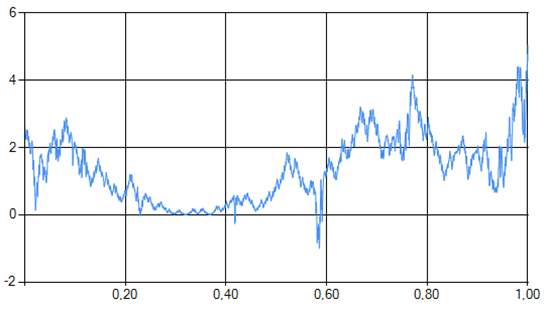
\includegraphics[width=0.8\textwidth]{fig1.png}
\label{fig1}
\caption{A figure caption.} 
\end{figure}



\begin{equation}
    \label{eq:18}
p'_i= \frac{ \log (p_i) - \log (p_{min})}{ \log (p_{max}) - \log (p_{min})} , 1 \leq i \leq k,
\end{equation}

\begin{figure}
\center
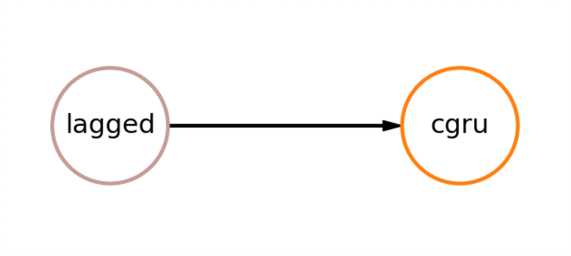
\includegraphics[width=0.8\textwidth]{fig2.png}
\label{fig2}
\caption{A figure caption.} 
\end{figure}


\section{Results of computational experiments}
\label{sec:5}


\begin{equation}
    \label{eq:19}
		\begin{matrix}
		  f(y)= -(AB + CD)^{1/2} \\
			AB =(\sum_{i=1}^7{\sum_{j=1}^7{[A_{ij} a_{ij} (y_1,y_2) + B_{ij} b_{ij} (y_1,y_2)])}})^2 \\
			CD =(\sum_{i=1}^7{\sum_{j=1}^7{[C_{ij} a_{ij} (y_1,y_2) - D_{ij} b_{ij} (y_1,y_2)])}})^2 \\
			a_{ij} (y_1,y_2) = \sin(\pi i y_1) \sin(\pi j y_2), \\
			b_{ij} (y_1,y_2) = \cos(\pi i y_1) \cos(\pi j y_2),
		\end{matrix}
\end{equation}


\begin{figure}
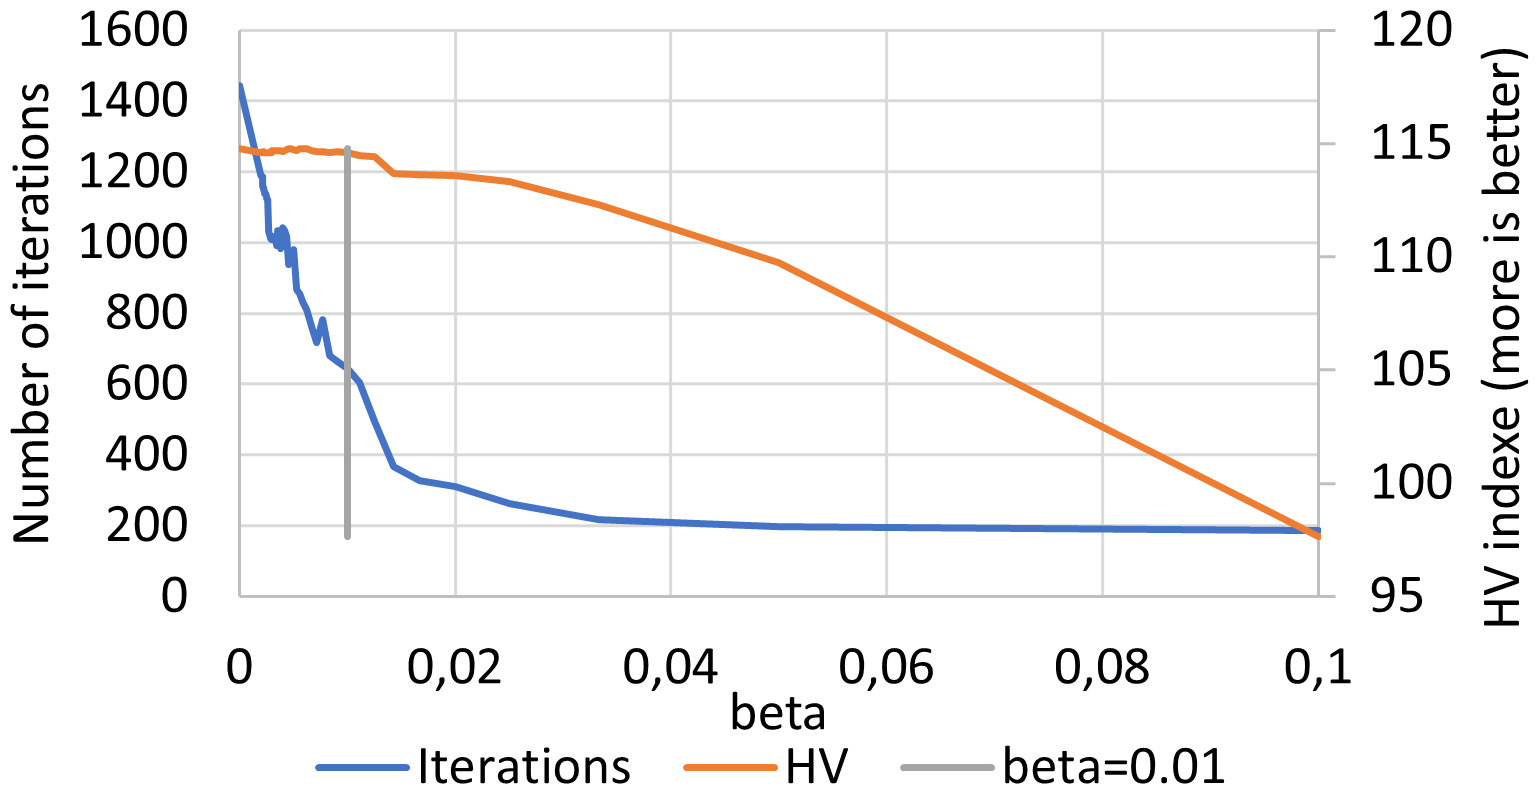
\includegraphics[width=\textwidth]{fig3.png}
\label{fig3}
\caption{A figure caption.} 
\end{figure}

\begin{figure}
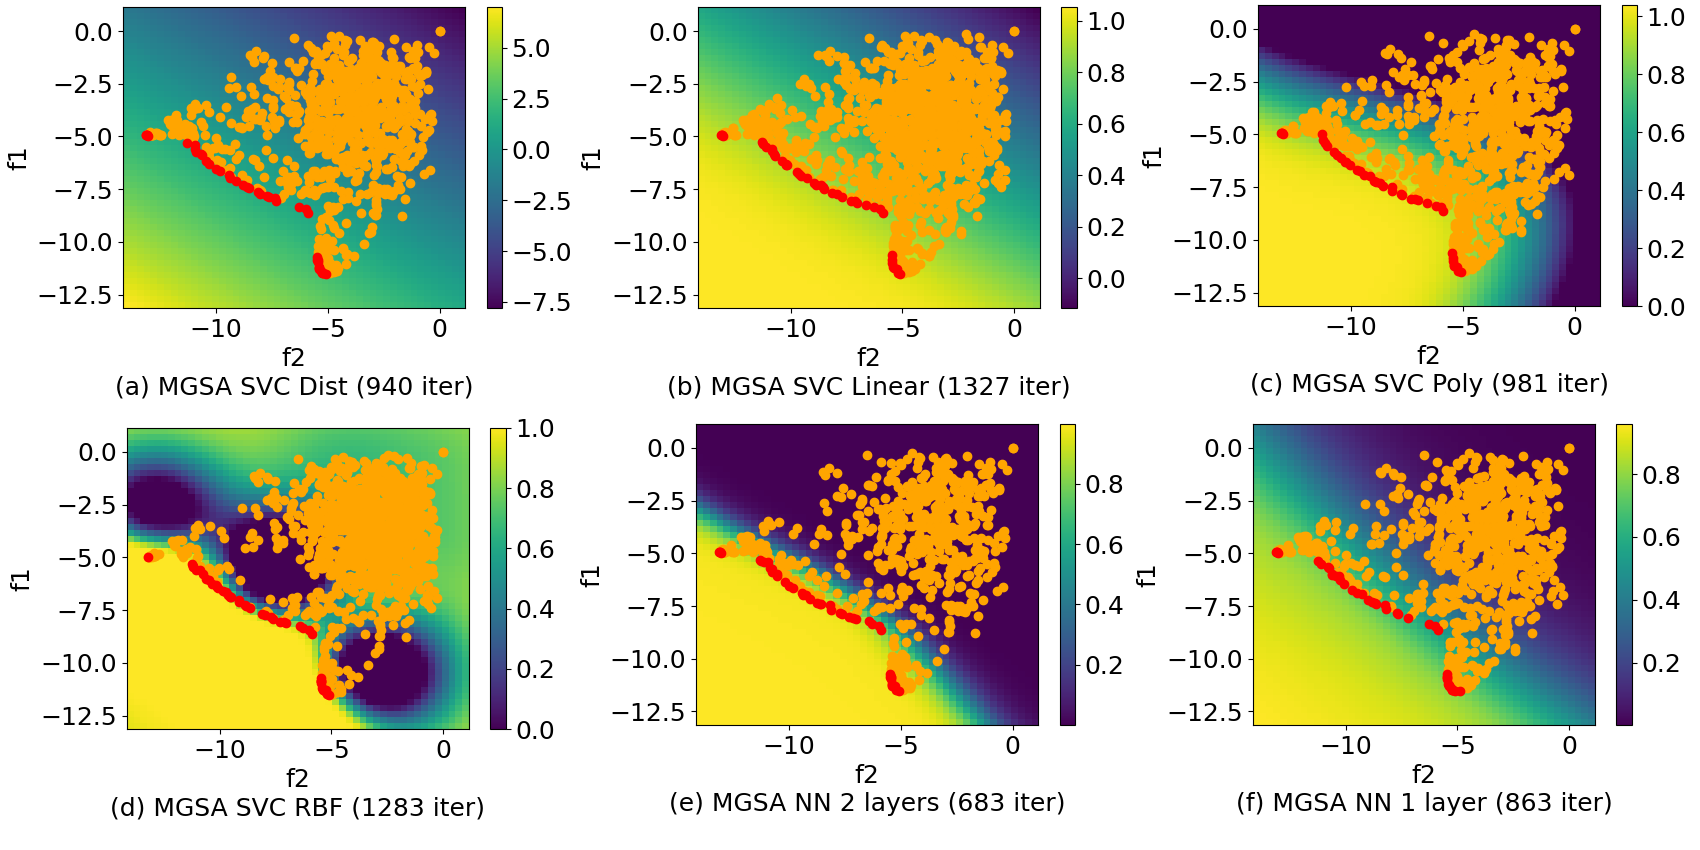
\includegraphics[width=\textwidth]{fig4.png}
\label{fig4}
\caption{A figure caption.} 
\end{figure}

\begin{figure}
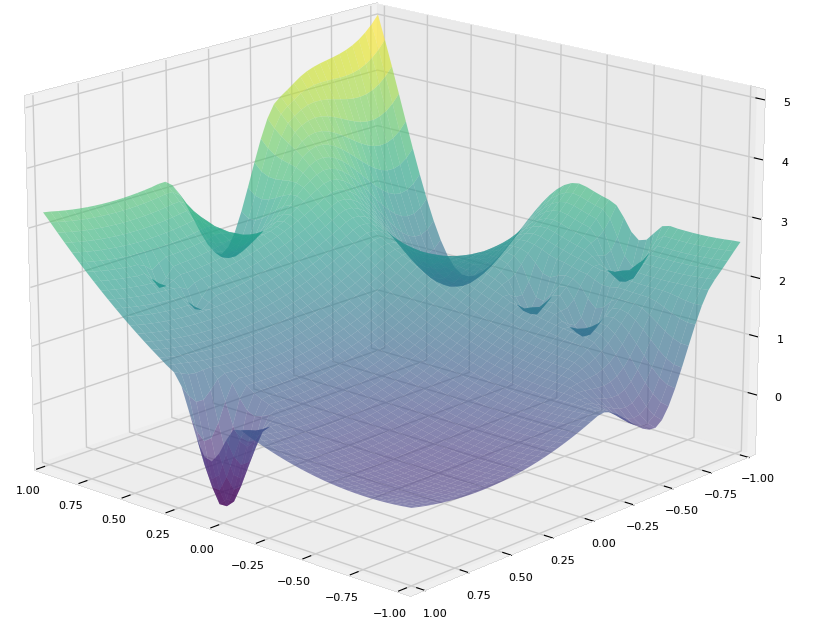
\includegraphics[width=\textwidth]{fig5.png}
\label{fig5}
\caption{A figure caption.} 
\end{figure}


%
% ---- Bibliography ----
%
% BibTeX users should specify bibliography style 'splncs04'.
% References will then be sorted and formatted in the correct style.
%
 \bibliographystyle{splncs04}
 \bibliography{bibliography}
%
%\begin{thebibliography}{8}
%\bibitem{ref_article1}
%Author, F.: Article title. Journal \textbf{2}(5), 99--110 (2016)
%
%\bibitem{ref_lncs1}
%Author, F., Author, S.: Title of a proceedings paper. In: Editor,
%F., Editor, S. (eds.) CONFERENCE 2016, LNCS, vol. 9999, pp. 1--13.
%Springer, Heidelberg (2016). \doi{10.10007/1234567890}
%
%\bibitem{ref_book1}
%Author, F., Author, S., Author, T.: Book title. 2nd edn. Publisher,
%Location (1999)
%
%\bibitem{ref_proc1}
%Author, A.-B.: Contribution title. In: 9th International Proceedings
%on Proceedings, pp. 1--2. Publisher, Location (2010)
%
%\bibitem{ref_url1}
%LNCS Homepage, \url{http://www.springer.com/lncs}, last accessed 2023/10/25
%\end{thebibliography}
\end{document}
